\section{Best responses and Nash Equilibria}
	\begin{definition}[Best response]
		A strategy $s^* \in S_i$ is a \textit{best response} of player $i$ to a
		strategy profile $s_{-i}$ if for every other strategy $t \in S_i$:
		\begin{equation}
			u_i(s_{-i}, s^*) \ge u_i(s_{-i}, t)
		\end{equation}
	\end{definition}
	
	$s^*$ is therefore the best choice for player $i$ given that the other
	players are playing strategies in $s_{-i}$. Player $i$ has no incentive to
	\textsc{unilaterally deviate} from $s^*$.

	Alternatively and equivalently,
	\begin{equation}
		u_i(s_{-i}, s^*) = \max \{ u_i(s_{-i}, t) \, | \, t \in S_i \} = \max_{t \in S_i} u_i(s_{-i}, t)
	\end{equation}

	\begin{definition}[Pure Strategy Nash Equilibrium]
		A strategy profile $s = (s_1, \ldots, s_n)$ is a Pure Strategy Nash
		Equilibrium (PNE) if for every player $i$, the strategy $s_i$ is a best
		response to $s_{-i}$.
	\end{definition}

	In other words, in $s = (s_1, \ldots, s_n)$ no player has an incentive to
	\textsc{unilaterally deviate}. A PNE is a strategy profile containing only
	best responses for each player.

	\begin{definition}[Mixed strategy]
		A \textit{mixed strategy} for player $i$ is a probability distribution
		over the set of pure strategies: $\sigma_i = (p(s_1), \ldots,
		p(s_{|S_i|})) \in \Delta^{S_i}$.
	\end{definition}

	The set of probability distributions
	$\Delta^{S_i} := \{ (x_1, \ldots, x_{|S_i|} ) \, : \, \sum_j ^{|S_i|} x_j =
	1 \land x_1, \ldots, x_{|S_i|} \ge 0 \}$ defines all probability
	distributions for player $i$'s strategies. A probability distribution
	$\sigma_i$ is a vector detailing the probabilities of player $i$ choosing
	each strategy $s \in S_i$, e.g. $\sigma_\text{I} = (\frac{1}{3}, 0,
	\frac{2}{3})$.

	\begin{definition}[Expected utility]
		Utility functions generalise from pure strategy profiles to mixed
		strategy profiles; the expected utlity for player $i$ under strategy
		profile $\sigma = (\sigma_1, \ldots, \sigma_n)$ is given by:
		\begin{equation}
			\label{eq:expectedUtility}
			u_i(\sigma_1, \ldots, \sigma_n) = \sum_{(S_1, \ldots, S_n) \in
			\mathcal{S}} \prod_j \sigma_j(s_j) \, u_i(s_1, \ldots, s_n)
		\end{equation}

	\end{definition}

	\begin{definition}[Mixed strategy best response]
		A mixed strategy $\sigma_i$ is a best response of player $i$ to a mixed
		strategy profile $\sigma_{-i}$ if:
		\begin{equation}
			u_i(\sigma_{-i}, \sigma_i) = \max_{\tau \in \Delta^{S_i}} u_i(\sigma_{-i}, \tau)
		\end{equation}
	\end{definition}

	\begin{definition}[Mixed strategy Nash Equilibrium]
		\label{def:BR}
		Strategy profile $\sigma = (\sigma_1, \ldots, \sigma_n)$ is a
		\textit{Mixed Nash Equilibrium} (MNE) if for every $i$, the strategy
		$\sigma_i$ is a best response to $\sigma_{-i}$.
	\end{definition}

	Hence in a MNE, no player has an incentive to unilaterally deviate.

\section{Finding Mixed Equilibria in $2\times2$ 2-player games}
	Suppose player I and II have two pure strategies $S_\text{I} = \{A, B\}$
	and $S_\text{II} = \{c, d\}$ respectively, and mixed strategies
	$\sigma_{\text{I}} = (p, 1-p)$ and $\sigma_{\text{II}} = (q, 1-q)$. That
	is, for example, player I plays strategy $A$ with probability $p$ and hence
	strategy $B$ with probability $1-p$ (and similarly for player II).
	Consider to following payoff matrix:
	\begin{center}
		\begin{tabular}{|c|c|c|}
			\hline
			I, II & $c$ & $d$ \\ \hline
			$A$ & 3,1 & 0,0 \\ \hline
			$B$ & 0,0 & 1,3 \\ \hline
		\end{tabular}
	\end{center}

	To compute the mixed equilibria of this game:
	\begin{enumerate}
		\itemsep0em
		\item Draw the diagram of best pure responses of player II to the mixed
			strategy $\sigma_{\text{I}} = (p, 1-p)$ of player I.
		\item Compute $p^* \in [0,1]$ which makes both pure strategies $c$ and
			$d$ best responses to $\sigma_{\text{I}}$ \footnote{Equivalently,
			find the mixed strategy $(p^*, 1-p^*)$ which makes player II
			\textit{indifferent} between $c$ and $d$.}.
		\item Repeat for player I
	\end{enumerate}

	In the above example, playing strategy $c$ player II gets expected
	payoff that ranges from 0 (at $p=0$) to 1 (at $p=1$). For strategy $d$
	player II's expected payoff ranges from 3 (at $p=0$) to 0 (at $p=1$).
	The resulting lines are shown in Fig. \ref{fig:expectedUtilityII} --
	these are straight lines due to linearity of expectation.
	\begin{center}
		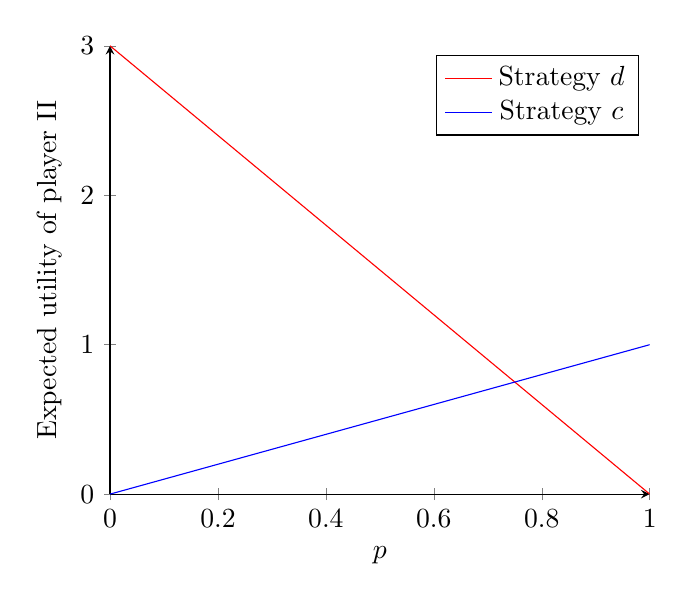
\begin{tikzpicture}
			\label{fig:expectedUtilityII}
			\begin{axis}[
					axis lines = left,
					xlabel = $p$,
					ylabel = {Expected utility of player II},
				]
				\addplot [
					domain=0:1,
					samples=100,
					color=red,
					]{-3*x+3};
				\addlegendentry{Strategy $d$}

				\addplot [
					domain=0:1,
					samples=100,
					color=blue,
				]{x};
				\addlegendentry{Strategy $c$}
			\end{axis}
		\end{tikzpicture}
	\end{center}

	Think of it this way: if player I plays strategy $A$ with increasing
	probability, and player II always plays $c$, player II's utility will
	increase from 0 to 1. Similarly, if player I plays strategy $A$ with
	increasing probability, and player II always plays $d$, players II's
	utility will fall from 3 to 0.

	These lines meet at point $p^*$, at which point player II is
	indifferent to his choice of strategy (both are best responses).

	For step 2, we have:
	\begin{equation*}
		\begin{split}
			\mathbb{E}[u_\text{I}((p^*, 1-p^*), c) & =
			\mathbb{E}[u_\text{I}((p^*, 1-p^*), d) \\
			1 p^* + 0 (1 - p^*) & = 0 p^* + 3 (1-p^*) \\
			p^* & = \frac{3}{4}
		\end{split}
	\end{equation*}

	Repeating for player I, we obtain the following graph:
	\begin{center}
		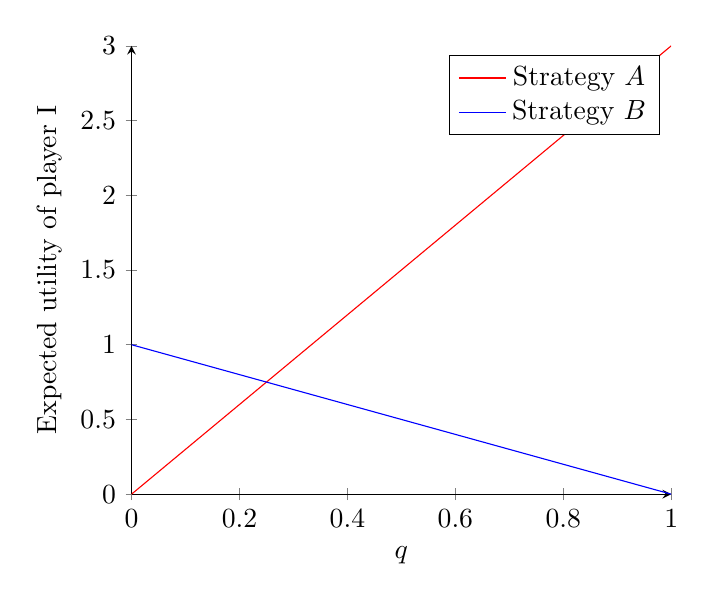
\begin{tikzpicture}
			\label{fig:expectedUtilityI}
			\begin{axis}[
					axis lines = left,
					xlabel = $q$,
					ylabel = {Expected utility of player I},
				]
				\addplot [
					domain=0:1,
					samples=100,
					color=red,
					]{3*x};
				\addlegendentry{Strategy $A$}

				\addplot [
					domain=0:1,
					samples=100,
					color=blue,
				]{-x+1};
				\addlegendentry{Strategy $B$}
			\end{axis}
		\end{tikzpicture}
	\end{center}

	Again: if player II plays $c$ with increasing probability and I always
	plays $A$, I's utility will increase from 0 to 3. If player II plays
	$c$ with increasing probability and I always plays $B$, I's utility
	will decrease from 1 to 0.

	These lines meet at $q^*$. Similarly to before, we can compute $q^*$ as before.
	Note that:
	\begin{equation}
		\begin{split}
			\mathbb{E}[u_\text{I}(A, (q^*, 1-q^*))] & = \mathbb{P}r[A] \mathbb{P}r[c] \, u_\text{I}(A,c) + \mathbb{P}r[A] \mathbb{P}r[d] \, u_\text{I}(A,d) + \mathbb{P}r[B] \mathbb{P}r[c] \, u_\text{I}(B,c) + \mathbb{P}r[B] \mathbb{P}r[d] \, u_\text{I}(B,d) \\
			& = \mathbb{P}r[A] \mathbb{P}r[c] \, u_\text{I}(A,c) + \mathbb{P}r[A] \mathbb{P}r[d] \, u_\text{I}(A,d)
		\end{split}
	\end{equation}

	The second line comes about as the probability of choosing $B$ in the
	mixed strategy $(1, 0)$ is 0, so we can disregard terms involving
	choosing $B$:
	\begin{equation*}
		\begin{split}
			\mathbb{E}[u_\text{I}(A, (q^*, 1-q^*)) & =
			\mathbb{E}[u_\text{I}(B, (q^*, 1-q^*)) \\
			3q^* & = 1 (1-q^*) \\
			q^* & = \frac{1}{4}
		\end{split}
	\end{equation*}

	Therefore, if such $p^*, q^* \in (0,1)$ exist, then the mixed strategy
	profile $((p^*, 1-p^*), (q^*, 1-q^*))$ is a truly mixed-strategy Nash
	Equilibrium.
